 \chapter{Clustering}

%%%%%%%%%%%%%%%%%%%%%%%%%%%%%%%%%%%%%%%%%%%%%%%%%%%%%%%%%%%%%%%%%%%%%%%%%%%%%%%%%%%%%%%%%%
\section{K-means}
\subsection{Choice of attributes and distance function}

We have selected $3$ attributes to performe the clustering via the K-Means algorithm.
In particular we have ignored the categorical attributes as there isn't a proper metric to define a distance function over these kinds of attributes.

The used attributes are only: \textit{limit}, \textit{ba\_mean}, \textit{pa\_mean}. Note that we have excluded the age in this list as it is the only one that isn't measured in NTD.

For these attributes we used the euclidean distance as metric function as it is more natural for this kind of attributes.

\subsection{Choise of the best value of k}

To choose the best value of $k$ we have plotted for each $K$ between $2$ and $50$ the values of the SSE and the silhouette score. Each value is calculated as the best among $10$ runs (with the lowest SSE) and with a maximum of $300$ iterations of the K-Means algorithm.

\begin{figure}[h]
  \begin{minipage}[h]{.50\textwidth}
    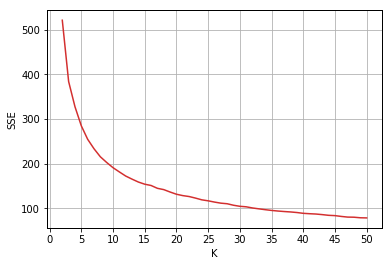
\includegraphics[width=1\textwidth]{img/ch3/kmeans_sse}
     \caption{SSE value for each $K$.}
  \end{minipage}
    \begin{minipage}[h]{.50\textwidth}
    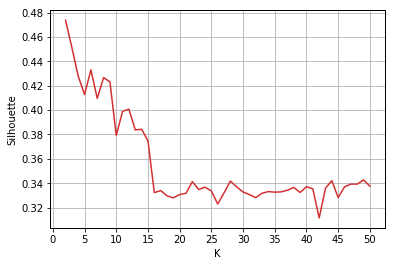
\includegraphics[width=1\textwidth]{img/ch3/kmeans_silhouette}
     \caption{silhouette score for each $K$.}
  \end{minipage}
\end{figure}

Using the elbow method we decide to set $k=6$ as it represents a good trade-off between SSE and data interpretability.

\subsection{Cluster analysis}

\begin{figure}[h]
  \begin{minipage}[h]{.40\textwidth}
    To better visualize the obtained clusters we have plotted the centers in parallel coordinates.
    
  From a first point of view we can see that all of the centers are separated in three class (low, medium, high) for all of the three used attributes.
  
  We want to go further in order to understand the different kind of customers and if there are some interesting correlation.
  \end{minipage}
    \begin{minipage}[h]{.60\textwidth}
    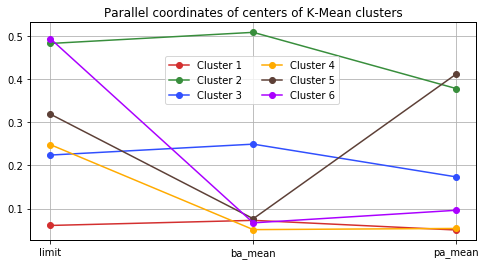
\includegraphics[width=.9\textwidth]{img/ch3/kmeans_center}
    %\caption{Attributes distribution over the clusters.}
  \end{minipage}
\end{figure}

\clearpage

\begin{figure}[h]
    \begin{minipage}[h]{.50\textwidth}
    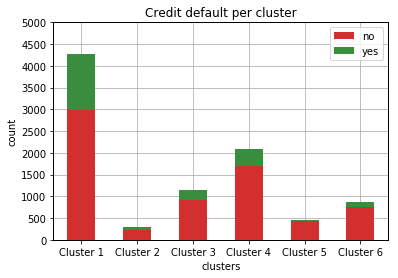
\includegraphics[width=1\textwidth]{img/ch3/kmeans_default}
    %\caption{Credit defaults in each cluster}

  \end{minipage}
  \begin{minipage}[h]{.50\textwidth}
    
    We have also plotted the number of credit defaults for each cluster to trying to understand the distribution of the customers. The cluster with the most credit default is the first one, with a ratio of $30\%$ and the cluster with the lowest credit default is the fifth, with a ratio of $6\%$.

  From the figures below we can see that the distributions of sex and status are the same for all the clusters, in particular their distributions are the same in the whole datasets so we can't use these attributes to make any assumptions over the obtained clusters.
      \end{minipage}
\end{figure}

\begin{figure}[h]
  \begin{minipage}[h]{.50\textwidth}
    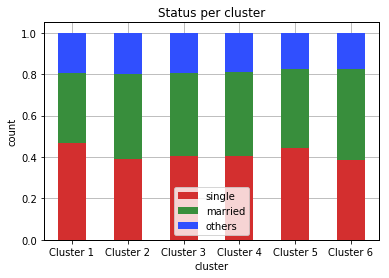
\includegraphics[width=1\textwidth]{img/ch3/kmeans_status}
  \end{minipage}
  \begin{minipage}[h]{.50\textwidth}    
    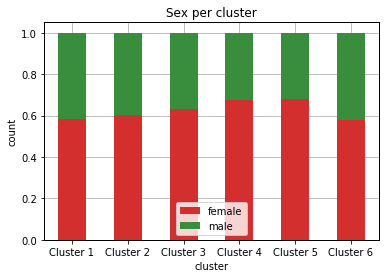
\includegraphics[width=1\textwidth]{img/ch3/kmeans_sex}
  \end{minipage}
\end{figure}

More useful are instead the distributions of the attributes relative to the educations and ages:

\begin{figure}[h]
  \begin{minipage}[h]{.50\textwidth}
    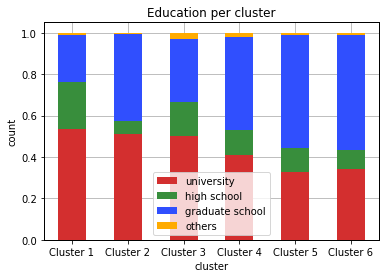
\includegraphics[width=1\textwidth]{img/ch3/kmeans_education}
  \end{minipage}
  \begin{minipage}[h]{.50\textwidth}    
    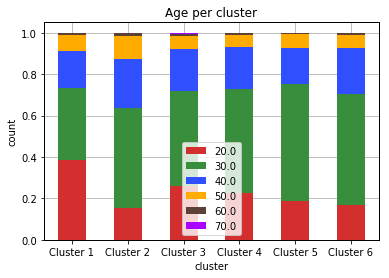
\includegraphics[width=1\textwidth]{img/ch3/kmeans_age}
  \end{minipage}
\end{figure}

We can discuss each cluster individually to see the most interesting properties.

\smallskip

\textcolor{red}{Cluster 1} is the biggest cluster, with $4276$ total elements include nearly half of the customers, and it is also the cluster with the highest credit default ratio ($40\%$). From the parallel coordinates plot we can see that the customers in this class have the credit cards with the lowest limit and also have the lowest bill/payment amounts over the six months. The lowest limit could be that this cluster is the one with most of young people ($40\%$ are below the $30$), but also is the cluster with most customer with an education in university and in high school. The high positive credit default ratio could be a combination of the distribution of these attributes (younger and university/high school).

\smallskip

\textcolor{green}{Cluster 2} with a total of $283$ customers is the smallest cluster. It has a credit default ratio of $21\%$ and it is the cluster with the older customers, nearly $40\%$ of the customers have an age higher that $40$. From the parallel coordinates we can see that is the only cluster with high limit and high bill amount and payment amount mean. 

\medskip

\textcolor{blue}{Cluster 3} has a total of $1143$ customers and a positive credit default ratio of $19\%$. In this cluster we have customers with a medium value of all the attributes.

\medskip

\textcolor{yellow}{Cluster 4} with a total of $2083$ customers is the second cluster for size and is has a positive credit default ratio of $21\%$. In this cluster we have customers with a medium credit card limit and with the lowest bill/payment amount mean.

\medskip

\textcolor{brown}{Cluster 5} has a total of $457$ customers and is the cluster with the lowest positive credit default ratio (only $6\%$). In this cluster we have customers with a credit card of medium limit, with a low bill amount mean but with the highest payment amount mean. From a point of view of the education in this cluster (and in the last cluster) we have the lowest number of education in university but the highest number of education in graduate school.

\medskip

\textcolor{violet}{Cluster 6} has a total of $879$ customers. It is the cluster with the highest limit in the credit cards but it has a low bill/payment amount mean.

\medskip

We decided to analize further the obtained cluster, so we separate the customers with a positive credit default from the customers with a negative credit default and plot all the normalized centers of the continuous attributes in two separated parallel coordinates plots: 

\begin{figure}[h]
  \begin{minipage}[h]{.50\textwidth}
    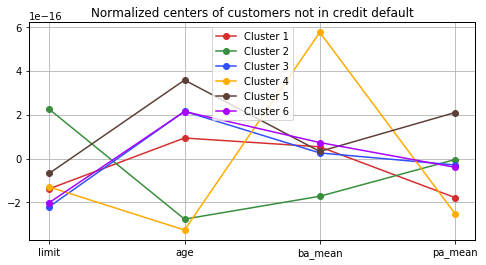
\includegraphics[width=1\textwidth]{img/ch3/kmeans_par_default_no}
  \end{minipage}
  \begin{minipage}[h]{.50\textwidth}    
    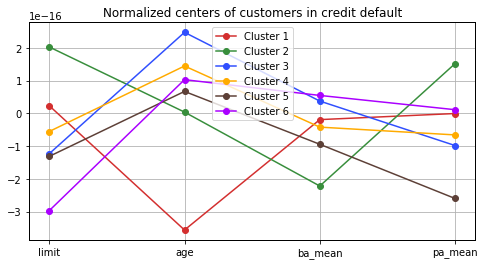
\includegraphics[width=1\textwidth]{img/ch3/kmeans_par_default_yes}
  \end{minipage}
\end{figure}

The most interesting cluster are \textcolor{red}{Cluster 1} and \textcolor{brown}{Cluster 5}, which are the ones with the highest and lowest positive credit default ratio, so we decided to analyze only these two clusters.

\medskip

For the \textcolor{red}{Cluster 1} the customers in credit defaults have an higher credit card limit and payment amount mean but a lower average age (compared to the customers not in credit default from the same cluster).

\medskip

For the \textcolor{brown}{Cluster 5} the customers in credit defaults have an higher credit card limit and payment amount mean but a lower average age (compared to the customers not in credit default from the same cluster).

%%%%%%%%%%%%%%%%%%%%%%%%%%%%%%%%%%%%%%%%%%%%%%%%%%%%%%%%%%%%%%%%%%%%%%%%%%%%%%%%%%%%%%%%%%
\section{DBSCAN}
\subsection{Choice of attributes and distance function}
\subsection{Study of the clustering parameters}
\subsection{Characterization and interpretation of the obtained clusters}
%%%%%%%%%%%%%%%%%%%%%%%%%%%%%%%%%%%%%%%%%%%%%%%%%%%%%%%%%%%%%%%%%%%%%%%%%%%%%%%%%%%%%%%%%%
\section{Hierarchical clustering}
\subsection{Choice of attributes and distance function}
\subsection{Discussion of dendograms using different algorithms}
%%%%%%%%%%%%%%%%%%%%%%%%%%%%%%%%%%%%%%%%%%%%%%%%%%%%%%%%%%%%%%%%%%%%%%%%%%%%%%%%%%%%%%%%%%

\section{Evaluation of clustering approaches and comparison of the clustering obtained}
